\graphicspath{{plots/}}
% JRM - revise abstract
\section{Introduction}

The increasing demand for high performance computing in data analysis, driven by
increasing data sizes and computational complexity, has rivaled that of scientific
computing in recent years \cite{fox:bdBenchmarking, kouzes:paradigm}. Many data analysts,
researchers, and scientists are turning to HPC machines to help with algorithms and tools,
such as machine learning, that are compuationally demanding and require large amounts of
memory \cite{raj:hpcBigData}. Many of the characteristics of large scale machines (e.g.
large amounts of RAM per node, high storage capacity, and advanced processing
capabilities) appear very attractive to these researchers, however, challenges remain for
many of the algorithms to make optimal use of the hardware \cite{lee:model}. Depending on
the nature of the analysis to be performed, analytics workflows may be carried out as many
independent concurrent processes requiring little or no coordination between them, or as
highly coordinated parallel processes in which the processes perform portions of the same
computational task. Examples of the former type of analysis include Monte Carlo
simulations and optimization problems with a parameter sweep through many different
initial conditions to compute an optimal result.  An example of the latter type of
analysis is the solution of large, sparse linear systems of such high order that the
computation of the solution can be effectively parallelized across the nodes. Regardless
of whether the workflow is implemented as independent concurrent or coordinated parallel
processes, it is important for data analysts to have software environments at their
disposal which can exploit the performance advantages of modern HPC machines.

Data analysts have come to rely heavily on the open source R programming environment to
manipulate and analyze their data. The R programming environment provides a language and
an interpreter designed around statistical computing \cite{ihaka:R}. The R language
interpreter is implemented in the C programming language, and the functionality of the
programming environment can be extended through packages that are commercially available
or available as open source. The ability to develop R packages in C means that developers
can extend the functionality of the environment and achieve high performance. This also
gives the R interpreter the flexability to link to external libraries optimized for
performance on a given system. As an example, the R environment can be compiled to
dynamically link with optimized instances of the BLAS \cite{dongarra:1990blas} and LAPACK
\cite{hammarling:1988blas} libraries for performing linear algebra computations.
Optimization of the R interpreter, its intrinsic functionality, and R packages for
specific hardware architectures will be necessary for data analysts to take full advantage
of the latest HPC clusters, and to obviate the need to reengineer their analysis workflows
in another language.

A way to assess the performance of software on a given computing platform and intercompare
performance across different platforms is through benchmarking. Benchmark results can also
be used to prioritize software performance optimization efforts on emerging HPC systems.
One such system is the Stampede 2 supercomputer at the Texas Advanced Computing Center
(TACC), which features the latest Intel Xeon Phi processors, codenamed Knight's Landing
(KNL). TACC and  Indiana University (IU) worked together on the Stampede project to
improve performance and scalilbity of applications using the R language on the original
Stampede machine. However, the original Stampde machine has a few key differences from
Stampede 2. The latest Intel Xeon Phi processor (KNL) is a many-core, vector processor
with up to 68 cores and two 512-bit vector processing units per core, a sufficient
deviation from the standard Xeon processors and Xeon Phi accelerators of the original
Stampede system to necessitate a performance assessment of the R programming environment
on both systems \cite{tacc:stampedeGuide}. While some work was done by both IU and TACC to
optimize R to run on the previous generation of Xeon Phi, codenamed Knight's Corner (KNC),
the number of real world R applications that could effectively make use of both the Xeon
Sandy Bridge processors (SNB) and the KNC accelerators was vanishingly small. For this
reason we focus our comparison of Stampde and Stampede 2 on comparing the KNL nodes and
only the SNB portion of the Stampede nodes.

We developed an R performance benchmark to determine the single-node run time performance
of compute intensive linear algebra kernels that are common to many data analytics
algorithms, and the run time performance of machine learning functionality commonly
implemented with linear algebra operations.  We then performed single-node strong scaling
tests of the benchmark on both Stampede systems to determine problem sizes and numbers of
threads for which the Stampede 2 nodes were comparable to or outperformed their original
Stampede counterparts.  It is our intention that the results be used to guide future
performance optimization efforts of the R programming environment to increase the
applicability of HPC machines like Stampede 2 to compute-intensive data
analysis.

The remainder of this paper as organized as follows, in section~\ref{sec:methodology} we
cover the design goals and capabilites of a new HPC R benchmark and discuss the
benchmarking strategy employed in the comparison between Stampede and Stampede 2.
section~\ref{sec:results} presents highlights of results from the benchmarking carried out
on the original Stampede and Stampede 2 machines, the implications and key lessons derived
from these results are detailed in section~\ref{sec:discuss}. Finally, we present our
conclusions and outline future work in section \ref{sec:future}.

\begin{table}
  \caption{HPC Microbenchmarks and Corresponding Kernel or Package Functions Tested}
  \label{tab:microbenchmarks}
  \begin{tabular}{ll}
    \toprule
    Microbenchmark & Kernel/Package function \\
    \midrule
    Cholesky factorization       & \texttt{chol} \\
    eigendecomposition           & \texttt{eigen} \\
    linear least squares fit     & \texttt{lsfit} \\
    linear solve w/ multiple r.h.s. & \texttt{solve} \\
    matrix cross product         & \texttt{crossprod} \\
    matrix determinant           & \texttt{determinant} \\
    matrix-matrix multiplication & $\%$$*$$\%$ \\
    matrix-vector multiplication & $\%$$*$$\%$ \\
    QR decomposition             & \texttt{qr} \\
    singular value decomposition & \texttt{svd} \\
    neural network training      & \texttt{nnet} \\
    cluster identification       & \texttt{pam} \\
    \bottomrule
  \end{tabular}
\end{table}

\section{Methodology and Approach}\label{sec:methodology}

To test the effiency and scalibility of the KNL system and compare to standard Xeon
architectures like SNB, we needed a flexible benchmark that could be easily scaled in
thread count and problem size and tested a variety of operations typical to R workflows.
When the most commonly used benchmarks in R did not meet our needs, we constructed a
framework and added several microbenchmarks that would meet our needs.

\subsection{A robust HPC benchmark for R} \label{sec:hpcBenchmark}

In our inital serach for a benchmark suite to use in our comparison of R performance on
Stampede and Stampede 2, we found that there are very few R performance benchmarks, and
there is no R performance benchmark that has been peer reviewed and accepted as a
standard. The most common and robust benchmark is the R Benchmark
\cite{urbanek:Rbenchmarks} which runs fifteen different microbenchmarks covering matrix
formation, matrix factorization, solving linear systems of equations, and sorting. Other
benchmarks like bench \cite{urbanek:Rbenchmarks}, for example, are microbenchmarks that
focus on a few specific computational kernels in R, but they lack the coverage needed to
comprehensively assess R performance in a high-performance computing environment. Although
R Benchmark is the most robust benchmark publicly available, it lacks the flexibility of
being able to easily adjust things like thread count and problem size, and it is focused
only on testing intrinsic functionality while leaving the performance of packages included
in the standard R distribution unassessed.  The benchmark is contained in a single R
function which times each R operation or function to be performance tested, but there is
no functionality to choose a specific operation or function to performance test.
Furthermore, the size of the input data to each test is hardcoded and there is no way to
loop over larger problem sizes as would be needed in scalability studies to test the
effectiveness of parallelism. Also, users of the benchmark cannot set the number of runs
over which to average the run time of a specific function without changing the number of
runs for all functions tested. The monolithic structure of R Benchmark also prevents
configuring the microbenchmarks to run concurrently in a cluster environment or to easily
choose select microbenchmarks to run independently.

When designing the benchmark, we wanted to maintain flexibility and extensibility while
still focusing in on the particular questions of interest for the comparison between
Stampede and Stampede 2. In particular we wanted to identify which R functions either
implemented multithreaded parallelism or could make use of underlying multithreaded
libraries; intercompare single-node run times and strong scaling on both the Sandy Bridge
and Knights Landing nodes; and be able to estimate the overhead incurred by R kernel
functions compared to similar kernel functionality implemented in C. Given that the kernel
functions are used as components in many machine learning and analytics algorithms, it was
important for us to determine which kernel functions performed poorly on the KNL
architecture compared to their performance on the SNB architecture. Furthermore, it was
worthwhile for us to run performance tests with similar kernel functionality exclusively
in C to determine the potential for performance improvement of the wrapper functions which
implement the kernels. In addition to performance testing the kernel functions, we tested
machine learning package functions to determine if and how those functions leverage any
parallelized kernels.

The HPC benchmark that we have developed performs microbenchmarking of compute-intensive
dense linear algebra kernels and packages that can utilize optimized linear algebra
kernels. We executed each microbenchmark with a wide range of problem dimensions and
thread counts to determine run time performance and scalability of the underlying R
functionality on each type of node, using strong scaling as the metric to determine
scalability for various thread counts. We chose dense linear algebra kernels for inclusion
in the benchmark because they form the computational foundation of many numerical methods
frequently utilized in R applications. The dense linear algebra kernels we included in the
benchmark are: Cholesky factorization, eigendecomposition, linear least squares fit,
linear solve with multiple right hand sides, matrix cross product, matrix determinant,
matrix-matrix multiplication, matrix-vector multiplication, QR factorization, and singular
value decomposition. All of the dense linear algebra kernels are implemented around BLAS
or LAPACK interfaces so the choice of optimized, multithreaded implementations of these
libraries and having them properly configured is crucial for performance.

We also included microbenchmarks of neural network training and cluster identification
functions from the \textit{nnet} and \textit{cluster} packages, respectively, that are
included in the standard R distribution. The \texttt{nnet} function is used to train
neural networks with a single hidden layer~\cite{ripley:pattern96}, and the \texttt{pam}
function, which implements the partitioning around medoids algorithm~\cite{chu:kmedoids,
reynolds:clustering}, is used to perform the cluster identification. We included benchmark
tests of these packages because neural network training and cluster identification can be
implemented with computational kernels tested in the benchmark. The neural network
training benchmark trains a neural network on a set of feature vectors drawn from a
multivariate normal distribution to approximate the probability density function from
which the vectors were drawn. We chose to approximate a multivariate normal probability
density function because the training problem is easy to scale in both number of training
vectors and number of features. The clustering benchmark generates normally distributed
clusters in an $N$-dimensional, real-valued feature space where the mean of one cluster is
located at the origin and the means of two clusters are each located at positions $-1$ and
$1$ of each axis.

We structured the HPC benchmark so that each kernel or package function is tested within
its own microbenchmark function. Table~\ref{tab:microbenchmarks} shows the kernels and
package functions tested by each microbenchmark. Each microbenchmark can be configured to
compute run time and performance for several problem sizes, where the run time with
respect to each problem size is computed as an average over a configurable number of runs
-- enabling users to test small problem sizes over a large number of runs to account for
operating system interference. Another advantage of implementing the microbenchmarks as
separate R functions is that they can be executed concurrently in cluster environments.

\subsection{Description of Tested Systems}

We conducted single-node performance tests on the SNB and KNL compute nodes of the
Stampede and Stampede 2 computing clusters, respectively. Each Sandy Bridge compute node
is a Dell PowerEdge C8220z with two eight-core, $2.7$~GHz Intel Xeon E5-2680 (Sandy Bridge
architecture) processors with $20$~MB of L2 cache each; $32$~GB of $1600$~MHz DDR3 RAM;
and a 61-core Intel Xeon Phi SE10P coprocessor (KNC). Each Knights Landing compute node is
a Dell PowerEdge with a single 68-core, $1.4$~GHz Intel Xeon Phi 7250 CPU (Knights Landing
architecture); $96$~GB of $2400$~MHz DDR4 RAM; and $16$~GB of on-package Multi-Channel
Dynamic Random Access Memory (MCDRAM) with $400$~GB/s bandwidth. Each of the Xeon Phi
cores has two 512-bit vector processing units which support a fused multiply-add
operation. The cores, which are grouped by tiles containing two cores and a shared $1$~MB
L2 cache~\cite{intel:xeonphi}, communicate with each other via a two-dimensional mesh
network to maintain cache consistency.

There are several different configuration options for the KNL architecture that are
determined by settings in the BIOS and can only be changed at boot time. These are whether
hyperthreading is enabled (when enabled there are four threads per core), the mode by
which the MCDRAM is accessed, and how the tiles are clustered together to access both the
MCDRAM and DDR4 RAM on cache misses~\cite{vladimirov:knlModes, asai:mcdramKnl}.  The
available options for MCDRAM access are flat mode, cache mode, and hybrid mode.  When the
KNL is in flat mode, applications can either explicitly allocate memory in MCDRAM via a
library like \textit{memkind}, or they can be run from MCDRAM using the command line
utility \texttt{numactl} to launch the application. Programs executed with
\texttt{numactl} allocate as much memory from MCDRAM as is available; any additional
memory needed by the program is allocated in main memory. When the CPU is in cache mode,
the MCDRAM acts as a level 3 cache, operating transparently to applications. We tested all
of the microbenchmarks in cache mode and a few in flat mode to compare performance in each
mode. We did not run any benchmarks in hybrid mode.

The KNL CPU can be configured in various clustering modes to group the tiles into
quadrants or hemispheres to take advantage of data locality in
applications~\cite{vladimirov:knlModes}. The options for clustering are all-to-all,
quadrant/hemisphere, and sub-numa clustering (SNC-2/SNC-4). All benchmarks were run in the
quadrant clustering mode.

Performance tests were conducted with the R programming environment version 3.2.1
downloaded from the Comprehensive R Archive Network. On the SNB nodes, running CentOS 6
(kernel 2.6.32-431.17.1.el6.x86\_64), we built the programming environment with the Intel
XE compiler versions 15.0 Update 2 (v. 15.0.2.164) and 17.0 Update 1 (v. 17.0.1.132), and
we linked the resulting executables with the parallel Intel Math Kernel Library (MKL)
versions 11.2.2 and 2017 Update 1, respectively. On the KNL nodes, running CentOS 7
(kernel 3.10.0-327.36.3.el7.xpps1\_1.4.1.3272.x86\_64), we built the programming
environment with the Intel XE compiler and linked with parallel MKL version 17.0 Update 1.
The \texttt{-xHost} compiler option was applied to both Sandy Bridge builds, and the
\texttt{-xMIC\_AVX512} option was applied to the Knights Landing build to utilize the
vector instruction set. The \texttt{xMIC-AVX512} option is needed to select the AVX-512
vector instruction set, the highest instruction set on Knights Landing, as the
\texttt{xHost} option is not supported for Xeon Phi processors. We passed the following
options to GNU Autoconf to generate shared R libraries and to link R with the MKL BLAS and
LAPACK libraries: \texttt{--without-x}, \texttt{--enable-R-shlib},
\texttt{--enable-shared}, \texttt{--with-blas}, and \texttt{--with-lapack}. The MKL
libraries provided the optimized and parallelized BLAS and LAPACK implementation
dependencies for all of our experiments. While there are many other options for optimized parallel BLAS and LAPACK libraries, we chose to focus our efforts on Intel's implementation of MKL.

The threading environment of each microbenchmark was configured through OpenMP and MKL
environment variables. As recommended in the MKL developer's guide~\cite{intel:mkl2017}
\texttt{KMP\_AFFINITY} was set to \texttt{KMP\_AFFINITY}=$granularity=fine,compact,1,0$.
We also disabled the dynamic thread adjustment controlled by \texttt{OMP\_DYNAMIC} and
\texttt{KMP\_DYNAMIC} so that the scaling tests could be conducted ~\cite{intel:cpp2015,
intel:cpp2017, intel:mkl11_2, intel:mkl2017}. The scalability of the microbenchmarks was
tested by increasing the number of MKL threads through the environment variable
\texttt{MKL\_NUM\_THREADS}.

% JRM - Justify thread counts
Hyperthreading was not enabled on the SNB processors, but it was enabled on the KNL
processors. We observed no improvements in scalability by placing more than one thread on
each core of the KNL processors, but have included results for more than 68 threads for
completeness. In fact, as shown in figure \ref{fig:knlScalabilityLimits}, increasing the
number of threads beyond the number of physical cores actually has a detrimental effect on
performance. The thread counts tested on the SNB nodes were: $1$, $2$, $4$, $8$, $12$, and
$16$; and the thread counts tested on the KNL nodes were: $1$, $2$, $4$, $8$, $16$, $34$,
$66$, $68$, $136$, $204$, and $272$. Small matrix dimensions of size $2000$ and $4000$
were often sufficient to determine performance cross over points for the linear algebra
kernels where one node type would begin to outperform the other given an increase in
matrix dimension. Larger matrices were useful for determining which kernels efficiently
utilized a large number of threads on the Knights Landing nodes. Apart from some
exceptions, we tested the linear algebra kernels with square matrices having the following
row dimensions $N$: $1000$, $2000$, $4000$, $8000$, $10000$, $15000$, $20000$, and
$40000$; in the case of the linear least squares fit kernel, the matrix dimensions were
$2N \times N/2$ for the same values of $N$. For each combination of matrix dimension and
number of threads for a given microbenchmark, we collected the run time and computed the
strong scaling as the ratio of the run time of the microbenchmark to the run time of the
microbenchmark with a single thread. We attempted to run performance tests up to matrix
dimensions of $30000$ and $40000$ on the Sandy Bridge and Knights Landing nodes,
respectively; however, some kernels could not be tested with these dimensions due to the
memory capacity and internal size limitations imposed by R.

The \texttt{nnet} was configured function so that several iterations of the underlying
solver would be required to optimize the neural net. The number of neurons in the hidden
layer (\texttt{size}) was set to $200$; the maximum number of solver iterations
(\texttt{maxit}) to $12500$; the absolute tolerance for the fit criterion
(\texttt{abstol}) to $1.0\times 10^{-6}$; the relative tolerance (\texttt{reltol}) to
$1.0\times 10^{-11}$; the flag enabling real-value outputs (\texttt{linout}) to
\texttt{TRUE}; and the maximum allowable number of weights (\texttt{MaxNWts}) to $4000$.
The \texttt{pam} function was executed with default parameters.

\section{Results} \label{sec:results}

Each of the microbenchmarks was run on both SNB and KNL for the matrix sizes and thread
counts enumerated in section \ref{sec:methodology}. This section outlines the results
obtained for the dense linear algebra benchmarks. In general, the results are for KNL
nodes with the MCDRAM operating in cached quadrant mode with hyperthreading enabled.
Additional results are presented for a small number of tests using different MCDRAM
configurations, different compiler configurations, and some additional results for higher
level machine learning packages \texttt{nnet} and \texttt{cluster}. We also implemented
and tested several equivalent microbenchmarks in C to determine the overhead incurred by R
functions calling MKL. While highlights are presented here, all of the results of the
tests can be obtained at {\bf NEED REFERENCE HERE!}.

% JRM - Do we want to reference the spreadsheet?
% SM - Somewhere around here, do you have a Scholarworks URL yet?
%The test results for each microbenchmark, matrix size, and number of threads are
%  given in a spreadsheet accompanying this document.

\subsection{Results from dense linear algebra microbenchmarks}

After running each of the microbenchmarks from table \ref{tab:microbenchmarks} for all of
the thread counts and matrix sizes on both KNL and SNB, we compared the run times and
scalability for each platform. For each microbenchmark we determined the minimum run time
over all tested numbers of threads. We computed the minimum run times in this manner for
each combination of node type, microbenchmark, and matrix dimension. From these minimum
values, we determined the fastest node type for each microbenchmark and matrix dimension
so that we could quantify relative performance. In the performance assessments that
follow, we provide the percentage of the maximum possible speedup, which we define as the
speedup divided by the number of physical cores (16 for SNB and 68 for KNL), achieved by
each microbenchmark with the largest matrix tested. We term this metric the efficiency as
it measures the percentage of linear speedup achieved for a microbenchmark. The results in
the following paragraphs are grouped by microbenchmarks that yielded similar performance
characteristics on SNB and KNL. Unless stated otherwise, the SNB performance assessments
are based on microbenchmarks built under the Intel 15 Update 2 bundle, and the KNL
performance assessments are based on microbenchmarks built under the Intel 17 Update 1
bundle.
\begin{figure}
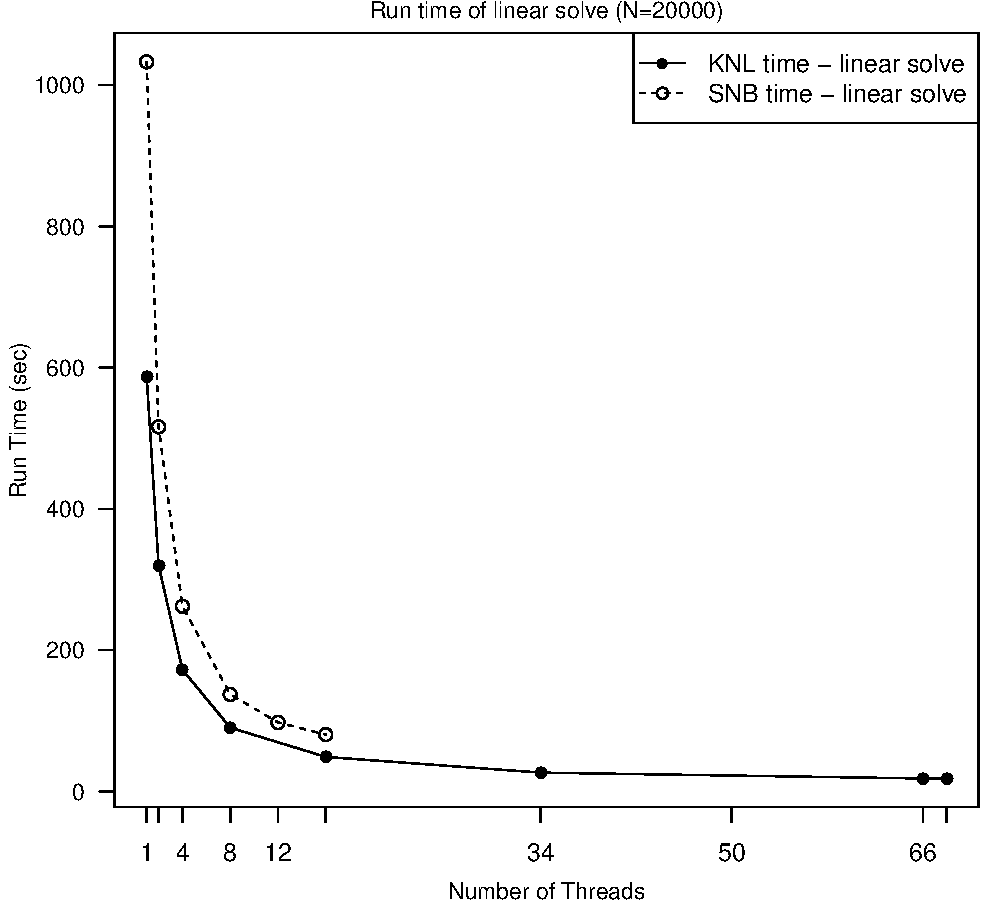
\includegraphics[height=\columnwidth, width=\columnwidth]{linsolve_20000_68-rt.pdf}
\caption{Run time of linear solve kernel for a large matrix.}
\label{fig:largeLinsolveTime}
\end{figure}

When comparing SNB performance to KNL we found that the SNB architecture could outperform
KNL for small matrix sizes. Several of the microbenchmarks, including Cholesky
factorization, linear solve, QR decomposition, and singular value decomposition (SVD) all
showed better performance on SNB for small matrix sizes, with a crossover in performance
to KNL occurring for moderate sized matrices, and KNL significantly outperforming SNB for
large matrix sizes. When looking at the best run times achieved by each node type, the SNB
nodes executed the Cholesky factorization up to $2.00$ times faster for tested matrix
sizes of $2000$ or smaller, the linear solve $1.77$ times faster for matrix size of
$1000$, and the matrix determinant $1.80$ times faster for matrix size of $1000$. However,
the KNL architecture began to outperform SNB for matrix sizes at or above $2000$ or $4000$
for the same kernels. In the best cases (i.e. the largest matrices), KNL achieved run
times that were $4.03$ (Cholesky factorization), $4.41$ (linear solve), and $5.23$ (matrix
determinant) times faster than those achieved on the SNB nodes given matrix dimensions of
$30000$, $20000$, and $40000$, respectively. Figure \ref{fig:largeLinsolveTime} shows the
run times for the linear solve microbenchmark for various thread counts on both SNB and
KNL with a matrix size of $20000$.

\begin{figure}
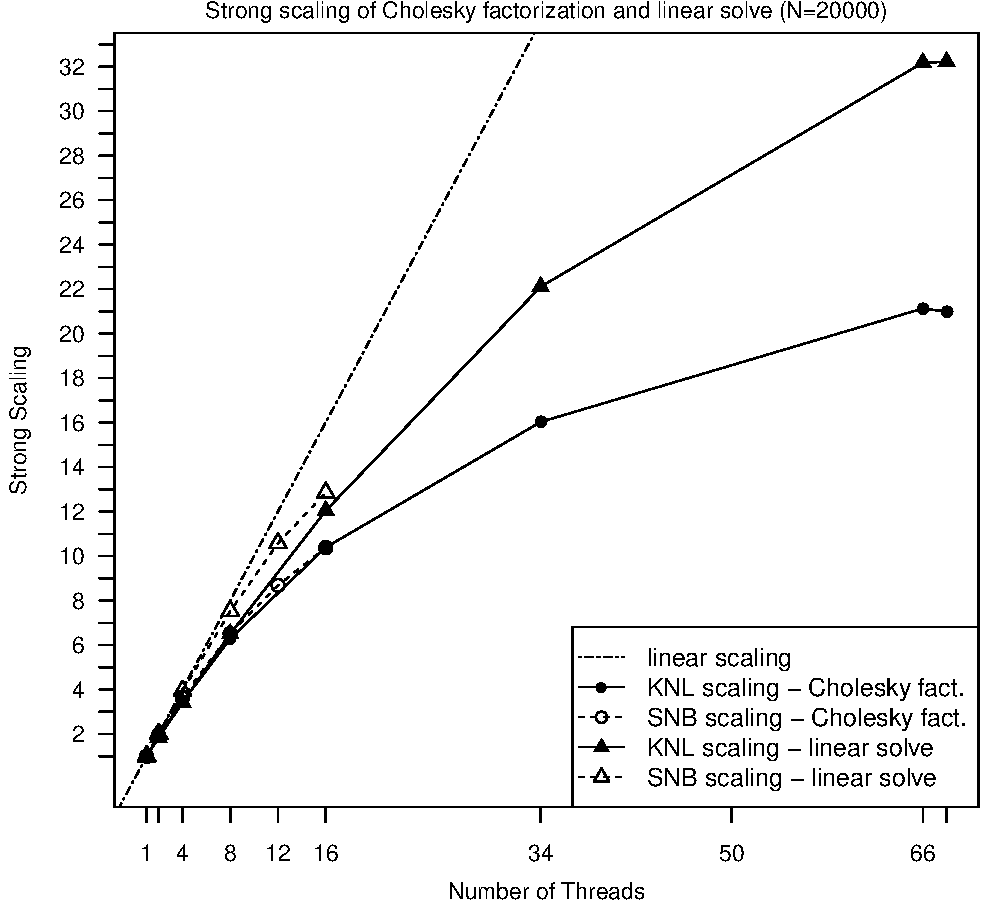
\includegraphics[height=\columnwidth, width=\columnwidth]{chol_solve_20000_68-ss.pdf}
\caption{.}
\label{fig:cholSolveScale}
\end{figure}

In terms of efficiency, the SNB nodes achieved $64\%$, $81\%$, and $84\%$ of the maximum
possible speedup with sixteen threads executing the Cholesky factorization kernel with
tested matrix dimensions of $30000$, the linear solve kernel with tested matrix dimensions
of $20000$, and the matrix determinant kernel with tested matrix dimensions of $40000$,
respectively. The KNL nodes achieved $38\%$, $48\%$, and $64\%$ of the maximum possible
speedup for the same kernels and matrix dimensions. While the KNL performance in terms of
run time is appreciably better than the SNB performance for large matrices, the efficiency
is not nearly as good when measured as a percentage of linear speedup, it is only by
virtue of the fact that there are so many more cores on KNL and the matrices are large
enough that the faster run times are achieved. This can be seen in the scalability curves
presented in figure \ref{fig:cholSolveScale} where the KNL results deviate from linear as
the core count increases toward the number of physical cores on the KNL.
\begin{figure}
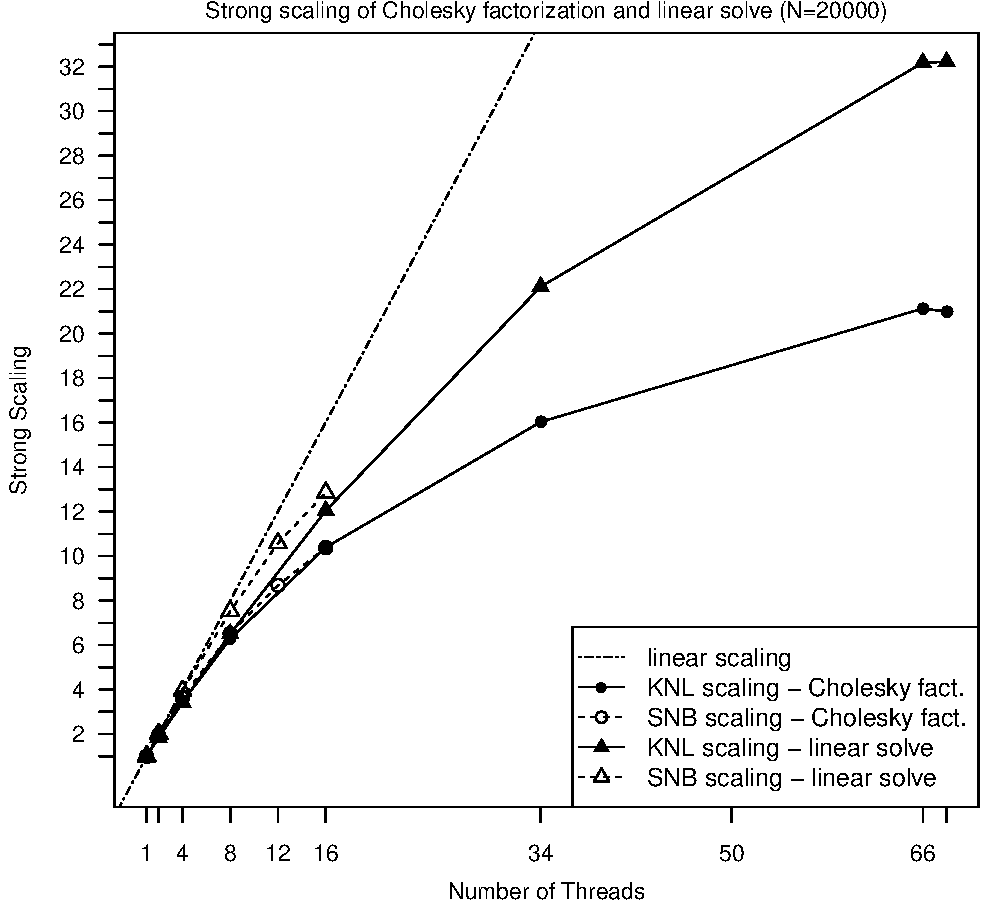
\includegraphics[height=\columnwidth, width=\columnwidth]{chol_solve_20000_68-ss.pdf}
\caption{Strong scaling of Cholesky factorization and linear solve kernels.}
\label{fig:cholSolveScale}
\end{figure}

The QR decomposition kernel, which calls the LAPACK \texttt{dgeqp3} routine, performed up
to $1.48$ times faster on the SNB nodes for matrix dimensions of $2000$ or less. For
matrix dimensions of $4000$ or more, the KNL nodes were up to $6.32$ times faster than the
SNB nodes. The KNL nodes achieved speedups of at most $28\%$ of the maximum possible, and
the SNB nodes achieved speedups of at most $38\%$ of the maximum possible. The SVD kernel
exhibited similar performance For each tested matrix dimension of $2000$ or less, the
kernel was up to $1.78$ times faster on SNB nodes than on KNL nodes. For tested matrix
dimensions of $4000$ or greater, the kernel was up to $4.25$ times as fast as on the SNB
nodes. The percentages of the maximum possible speedup achieved by the KNL and SNB nodes
were at most $23\%$ and $22\%$, respectively.
\begin{figure}
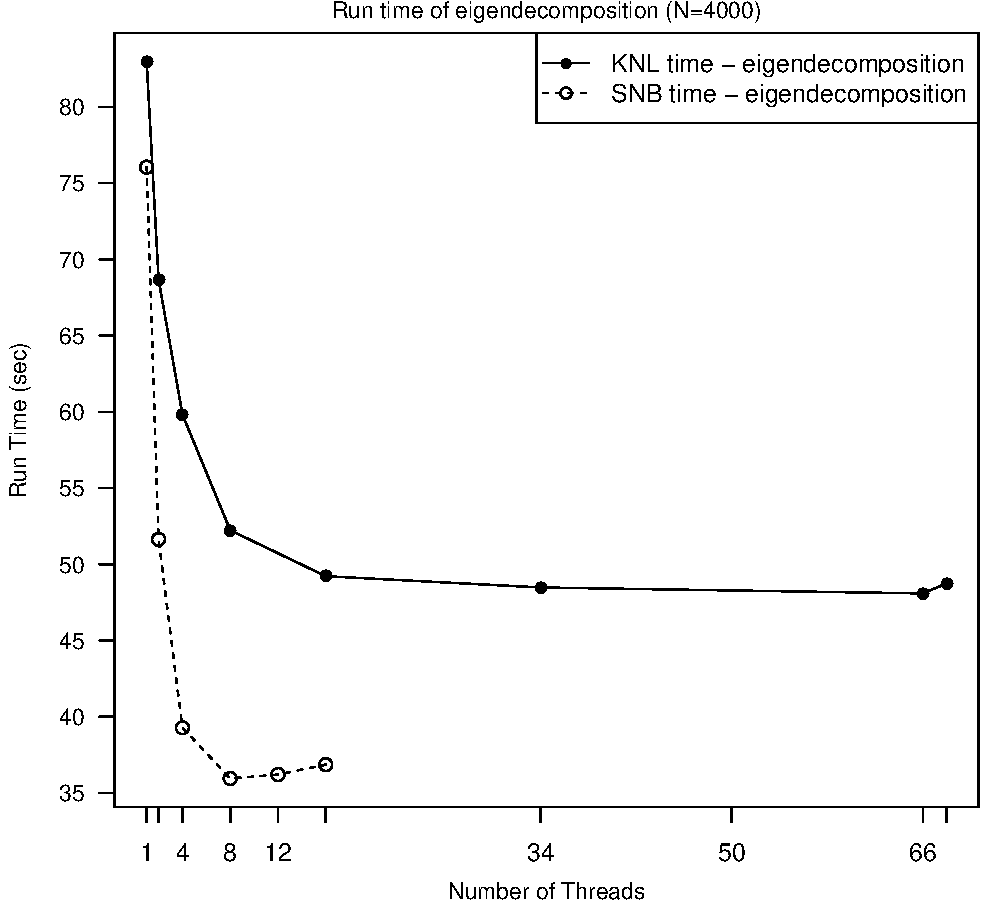
\includegraphics[height=\columnwidth, width=\columnwidth]{eigen_4000_68-rt.pdf}
\caption{Run time of eigendecomposition kernel for medium sized matrix.}
\label{fig:mediumEigenTime}
\end{figure}

Both the eigendecomposition and linear least squares kernels exhibited issues with scaling
to higher thread counts on both SNB and KNL. In general, the SNB nodes performed better
overall for these two kernels. The eigendecomposition kernel performed up to $2.75$ times
faster on the SNB nodes than on the KNL nodes for tested matrix dimensions of $8000$ or
less. As we increased the matrix dimension beyond $8000$, the KNL nodes were up to $1.54$
times faster than the SNB nodes. For tested matrix dimensions of $20000$ or less, the KNL
nodes achieved at most $5\%$ of the maximum possible speedup, and the SNB nodes achieved
at most $17\%$ of the maximum possible speedup. The eigendecomposition kernel never scaled
beyond eight threads on the SNB nodes, regardless of matrix dimension, but the performance
did not deteriorate as the maximum number of threads (sixteen) was reached either. The
performance characteristics for various thread counts with matrix size $4000$ can be seen
in figure \ref{fig:mediumEigenTime}. The linear least squares fit kernel experienced
difficulties scaling beyond four threads on the SNB nodes. The SNB run times were up to
$2.18$ times faster than those of the KNL nodes for tested values of $N=8000$ or less, and
the SNB nodes achieved at most $10\%$ of the maximum possible speedup for tested values of
$N=20000$ or less. The KNL run times were up to $1.46$ times faster than the SNB nodes for
tested matrix sizes greater than $8000$. The strong scaling on KNL nodes stagnated beyond
eight threads, achieving only $5\%$ of the maximum possible speedup for tested values of
$N=20000$ or less.

For the matrix cross product and matrix-matrix multiplication microbenchmarks the KNL
nodes had equal or greater performance than the SNB nodes for all matrix dimensions and
numbers of threads tested. The matrix cross product kernel was up to $4.27$ times faster
on the KNL nodes than on the SNB nodes for tested matrix dimensions of $40000$ or less.
The matrix-matrix multiplication kernel was up to $3.12$ times as fast on the KNL nodes
than on the SNB nodes for tested matrix dimensions greater than $2000$. The KNL and SNB
nodes executing the matrix cross product kernel achieved $51\%$ and $84\%$ of their
maximum possible speedups, respectively. The KNL and SNB nodes executing the matrix-matrix
multiplication kernel achieved $43\%$ and $96\%$ of their maximum possible speedups,
respectively. Timing results for matrix-matrix multiplication with matrix size $N=20000$
are given in Figure~\ref{fig:largeMatmatTime}.
\begin{figure}
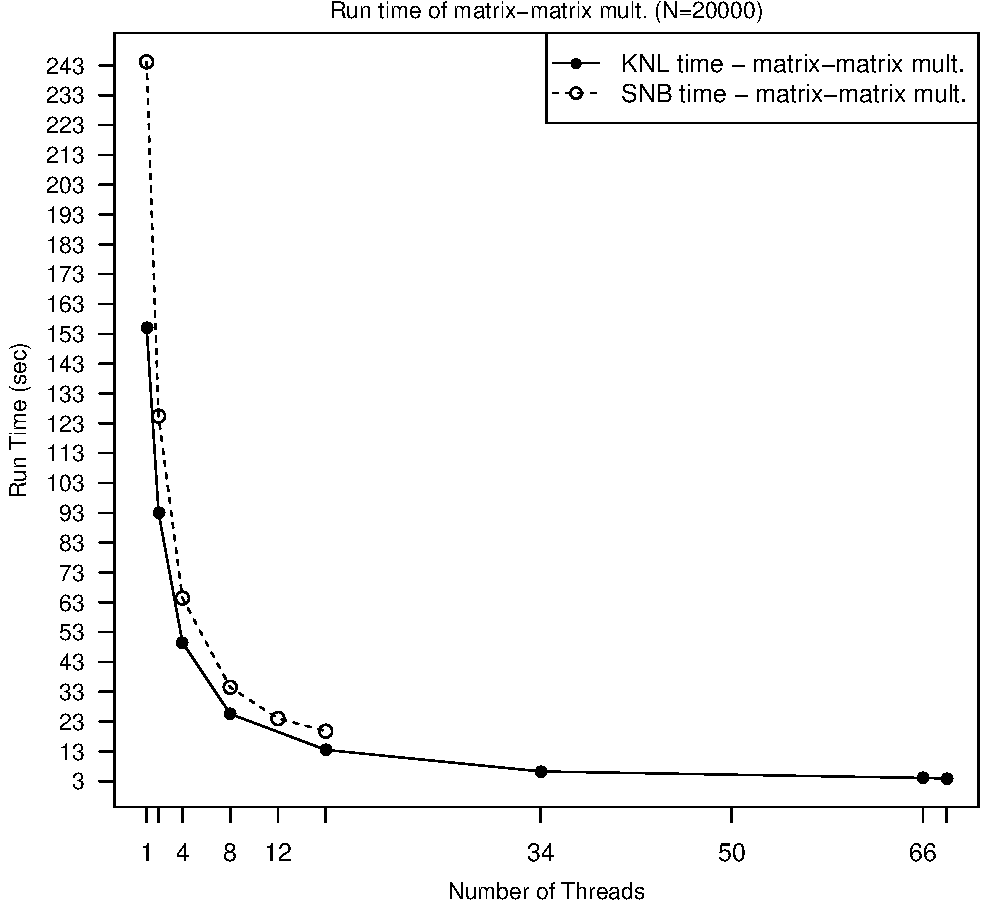
\includegraphics[height=\columnwidth, width=\columnwidth]{matmat_20000_68-rt.pdf}
\caption{Run time of matrix-matrix multiplication kernel for large matrix.}
\label{fig:largeMatmatTime}
\end{figure}

The matrix-vector multiplication kernel on the SNB nodes consistently outperformed the KNL
nodes for all tested matrix dimensions and numbers of threads. The kernel was up to $6.14$
times faster on the SNB nodes than the KNL nodes for matrix dimensions of $40000$ or less.
The speedups achieved by the KNL and SNB nodes with the kernel were at most $2\%$ and
$9\%$ of the maximum possible, respectively.

\subsection{Additional results}

We also tested the performance of the Cholesky factorization, linear solve, and matrix
cross product kernels when run exclusively out of the high-bandwidth MCDRAM. This was
accomplished by executing the kernels on KNL nodes booted in flat mode and using the
\texttt{numactl} utility with the \texttt{--preferred} option to indicate that as much
memory as possible for the R programming environment was to be allocated in the MCDRAM
NUMA node; the environment and the dynamically allocated matrices we tested fit entirely
in MCDRAM. The performance results showed no appreciable differences in kernel performance
when the MCDRAM was configured in cache mode or flat mode.

We conducted additional experiments with the SNB nodes to determine if the linear least
squares fit, linear solve, or QR decomposition microbenchmarks would show improvement
under the Intel 17 Update 1 compiler and MKL. The linear solve and QR decomposition
microbenchmark results showed little or no improvement over their Intel 15 Update 2
counterparts; however, the linear least squares fit exhibited improved scalability beyond
four threads for moderate to large matrix dimensions.

We also tested the \texttt{nnet} function from the \textit{nnet} package and the
\texttt{pam} function of the \textit{cluster} package to determine if those capabilities
were parallelized. Our tests revealed that neither of the package functions was
parallelized, as was indicated by the run times and the analysis tools we used to
determine if multiple threads were being created. The SNB nodes were approximately $3.5$
times faster and $3.0$ times faster than the KNL nodes at training the neural network with
three features and five features (Table~\ref{tab:nnetResults}), respectively. Note that
the run times decreased when we increased the number of feature vectors from $5000$ to
$10000$ and the feature vector was of dimension three. This is because neural network
training solves a non-convex objective function that can vary greatly with the number of
training vectors and features; therefore, it is useful only to compare performance between
the two node types for a pair of features and number of training vectors. The SNB nodes
were approximately $1.34$-$1.44$ times faster than the KNL nodes when running the
\texttt{pam} function for up to $17500$ feature vectors, but the KNL nodes closed that gap
to approximately $1.04$ times as fast for $35000$ feature vectors. With $40005$ feature
vectors, the KNL nodes were $1.11$ times faster than the SNB nodes.

% Neural networking benchmark results
\begin{table}
  \caption{Run Time of Neural Network Training Benchmark}
  \label{tab:nnetResults}
  \begin{tabular}{llcc}
    \toprule
      Number of & Number of training & \multicolumn{2}{c}{Run time (sec)}\\
      features  & vectors            & SNB & KNL\\
    \midrule
    $3$ & $5000$  & $3.239\times 10^{2}$ & $1.041\times 10^{3}$ \\ % SNB
    $3$ & $10000$ & $1.842\times 10^{2}$ & $6.736\times 10^{2}$ \\ % SNB
    $5$ & $5000$  & $3.520\times 10^{2}$ & $1.031\times 10^{3}$ \\ % SNB
    $5$ & $10000$ & $1.536\times 10^{3}$ & $4.912\times 10^{3}$ \\ % SNB
    %$5$ & $15000$ & $2.660\times 10^{3}$ & $8.216\times 10^{3}$ \\
    \bottomrule
  \end{tabular}
\end{table}

% Clustering benchmark results
\begin{table}
  \caption{Run Time of Clustering Benchmark}
  \label{tab:clusterResults}
  \begin{tabular}{lllcc}
    \toprule
    Num. of   & Num. of   & Num. of & \multicolumn{2}{c}{Run time (sec)}\\
    features  & clusters  & feature           & SNB & KNL\\
              &           & vectors           & &\\
    \midrule
    %$3$ & $7$ & $7000$  & $4.416\times 10^{1}$ & $5.949\times 10^{1}$ \\
    %$3$ & $7$ & $10500$ & $1.065\times 10^{2}$ & $1.536\times 10^{2}$ \\
    $3$ & $7$ & $14000$ & $2.890\times 10^{2}$ & $4.134\times 10^{2}$ \\ % SNB
    $3$ & $7$ & $17500$ & $6.757\times 10^{2}$ & $9.324\times 10^{2}$ \\ % SNB
    $3$ & $7$ & $35000$ & $2.578\times 10^{3}$ & $2.689\times 10^{3}$ \\ % SNB
    $3$ & $7$ & $40005$ & $9.236\times 10^{3}$ & $8.313\times 10^{3}$ \\ % SNB
%    $16$ & $33$ & $40029$ &                    & $1.4245\times 10^{4}$ \\ % SNB
    \bottomrule
  \end{tabular}
\end{table}


The overheads in the linear algebra kernel functions, all of which call BLAS or LAPACK
routines to perform the bulk of the computation~\cite{cran:Rmanuals}, can potentially be
large compared to similar functionality implemented exclusively in C due to data copying
and validity checking that is common in interpreted languages. To determine the potential
for further optimization of R functionality, we developed a set of drivers for the matrix
cross product, QR decomposition, and linear solve in C and compared their performance to
their their R internal function counterparts. The cross product internal function is
implemented as a call to the LAPACK FORTRAN function \texttt{dsyrk} followed by a for loop
to copy the upper triangle of the result matrix to its lower triangle; the C driver
replicates this behavior. The QR decomposition internal function is implemented as a call
to the LAPACK FORTRAN function \texttt{dgeqp3}, and the dense linear solve internal
function is implemented as a call to the LAPACK FORTRAN function \texttt{dgesv}. The C
driver for QR calls the \texttt{LAPACKE\_dsyrk} C wrapper function which dynamically
allocates an optimally sized workspace, the other driver functions call the FORTRAN
functions directly. The R implementation of the linear solve computes an estimate of the
condition number by default, a task we did not implement in the corresponding C driver.
The results showed that the performance of R internal functions are highly competitive
with the native C drivers for all matrix dimensions and threads. The performance curves
for the dense linear solve applied to the smallest tested matrix dimensions do
show some performance anomalies, however. There is a substantial difference between the
strong scaling of the C driver and the R kernel when using two threads. Furthermore, the C
driver scalability diverges sharply from that of the R kernel for eight or more threads
for matrix dimensions $1000$ and $2000$. We reran the strong scaling test of the C driver
several times for the smaller matrix dimensions to verify the results, with no appreciable
change in the curves.

%SM -- Need either a plot or max deviation numbers here. Quantify ``highly competitive" and ``substantial difference''

\section{Discussion} \label{sec:discuss}

\begin{figure}
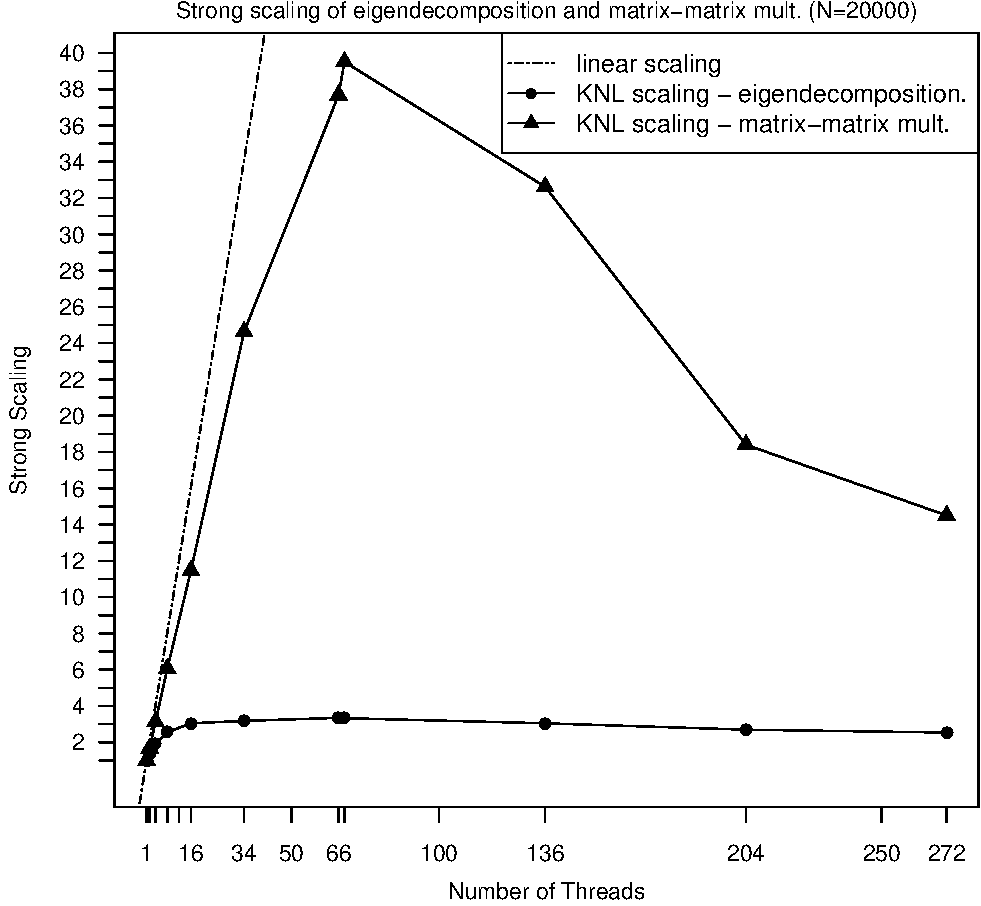
\includegraphics[height=\columnwidth, width=\columnwidth]{eigen_matmat_20000_272_knl-ss.pdf}
\caption{Limits of KNL scalability for two kernels}
\label{fig:knlScalabilityLimits}
\end{figure}

We developed a new R HPC benchmarking package consisting of microbenchmarks of several
computational kernels and benchmarks of machine learning functions from the standard R
distribution. The implementation of the benchmarks improves upon limitations of the few R
benchmarks that have been developed to date, namely the inability to perform scalability
studies over successively larger problem sizes and to independently configure how each
individual benchmark is executed. With few exceptions, the SNB nodes achieved the best run
time performance for matrix dimensions up to a few thousand, an expected result given that
the small problem sizes limit scalability on the KNL nodes and that the clock speed of the
SNB CPUs is roughly twice that of the KNL CPUs. However, the best run time achieved on the
SNB nodes was never more than three times as fast as the best run time achieved on the KNL
nodes for a given matrix dimension, except in the case of matrix-vector multiplication,
for which the SNB nodes were over six times faster than the KNL nodes. The poor
scalability of the matrix-vector kernel may be because the single-core performance is very
high and matrices of larger dimension could not be tested to increase the workload per
core due to limitations on matrix dimensions imposed by R and memory allocation failures
that occurred.

When we tested the Cholesky factorization, linear solve, matrix determinant, matrix-matrix
multiplication, and matrix cross product kernels, the KNL nodes achieved strong scaling
speedups of up to $45$ times their single-threaded performance for large matrices.
Furthermore, the KNL nodes were up to $5.25$ times faster than the SNB nodes for the same
kernels and the largest matrix dimensions. KNL was also $6.5$ times faster than the SNB
architecture for QR and singular value decompositions for the largest tested matrix
dimensions, and the KNL nodes achieved strong scaling speedups of up to $19$. The KNL
nodes achieved modest strong scaling speedups of up to $3.5$ for large matrix dimensions
when we tested them with the eigendecomposition and the linear least squares fit kernels.
Due to the limited scalability of these kernels, the KNL nodes were only about $1.5$ times
faster than the SNB nodes.

In summary, we were able to draw five important conclusions from our research.
\begin{enumerate}
\item Strong scaling flattens past 68 threads for the benchmarked linear algebra kernels,
which heavily leverage the linear algebra routines of MKL. As evidenced in figure
\ref{fig:knlScalabilityLimits}, we saw that increasing the thread count beyond the
physical number of cores did not provide any benefit to performance, and in many cases,
was detrimental to performance. The plot of strong scaling shows results for up to $272$
threads on the KNL node to show how strong scaling decreases after more threads than the
number of cores are applied, a performance characteristic that was true of all of the
matrix kernels we tested. In the best cases we saw results similar to those for
eigendecomposition shown in figure \ref{fig:knlScalabilityLimits} where the scalability
flattens and the run time does not improve with increasing thread count. However, in the
worst cases, such as matrix-matrix multiplication shown in figure
\ref{fig:knlScalabilityLimits} the performance actually decreases substantially when
increasing thread count.

\item The matrices must be large enough to provide sufficient work for scalability. In
general, to make full use of the large core count and wide vector units of KNL, one needs
to be operating on large matrices. We typically saw that for matrices of about $4000\times
4000$ or less in size, the SNB nodes performed better than the KNL nodes. However, as the
matrix sizes were increased the KNL nodes outperformed the SNB nodes by as much as a
factor of five.

\item The R interpreter overhead is negligible for microbenchmarked functions. By
comparing the R implementation to a functionally similar kernel drivers implemented in C,
we found that the overhead incurred by the R interpreter is negligible.

\item The MCDRAM flat mode does not offer any performance benefit over cached mode. The
performance overhead of cached mode was negligible for our particular tests. However, our
tests did not include any long-running simulations or benchmarks, so they were not
affected by memory fragmentation. Also, it should be noted that the largest matrices we
tested would fit entirely in MCDRAM, so we were not evaluating MCDRAM as a cache device in
larger or longer-running calculations.

\item Finally, many higher level R packages are not properly structured to take full
advantage of the many-core, vectorized architecture of the Xeon Phi, and they do not
leverage the MKL functionality exposed in the microbenchmarked functions. The two
higher-level packages we tested, \textit{nnet} and \textit{cluster}, did not perform
particularly well on KNL when compared to SNB. And although it is certainly possible to
implement these algorithms using the functions we tested in the linear algebra kernel
microbenchmarks via MKL or some other optimized linear algebra libraries, it appears that
these implementations do not exercise this option.

\end{enumerate}

\section{Future Work} \label{sec:future}
Based on the conclusions presented in section \ref{sec:discuss} there are several areas
where extension of the current work is warranted. First, the suite of microbenchmarks
implemented in this first version of our R benchmark focuses heavily on fairly low level
dense matrix operations. This was a deliberate choice as these functions were most likely
to run optimally on the KNL architecture. However, the R ecosystem is quite broad and it
is reasonable to include additional focus benchmark areas. Fortunately, owing to the
design of the benchmarking framework this is not difficult to do. We will work to extend
the benchmark to include sparse linear algebra kernels from the \textit{matrix} library,
and summary statistics kernels such as mean, variance, and covariance computation.

Additional compute intensive machine learning or data analytics functionality commonly
used in R should eventually be included in the benchmark to provide more extensive
performance assessments. If the performance of the \textit{nnet} and \textit{cluster}
packages are an indication of the performance of R packages in general, packages will
likely need to be vectorized and either parallelized or restructured to take full
advantage of the KNL architecture. It should also be noted, that the trend toward higher
amounts of vectorization and parallelization is not unique to KNL. Efforts to improve R
functionality along these lines will likely meet with improved performance on any
architecture.

The benchmarking framework and suite presented here is currently being packaged for inclusion into CRAN, the Comprehensive R Archive Network. This will allow the benchmark to be used more widely and will allow for R performance data to be collected more easily and in a standardized way.

\begin{acks}
%  The authors would like to thank...
%  See also \grantsponsor and \grantnum commands in acmguide.pdf
This work was supported in part by the \grantsponsor{GSACI1134872}{National Science Foundation}{http://www.nsf.gov} through award \grantnum[https://www.nsf.gov/awardsearch/showAward?AWD\_ID=1134872]{GSACI1134872}{ACI-1134872} to the Texas Advanced Computing Center (TACC) at The University of Texas at Austin.
%\grantsponsor{GSNSFACI1134872}{National Science Foundation}{http://www.nsf.gov}
%\grantnum[https://www.nsf.gov/awardsearch/showAward?AWD_ID=1134872]{GSNSFACI1134872}{ACI-1134872}
\end{acks}

\bibliographystyle{ACM-Reference-Format}
\bibliography{PEARCKNL}
